% !BIB TS-program = biber

\RequirePackage[l2tabu,orthodox]{nag}

% TODO: decide if one-sided/two-sided
%\documentclass[headsepline,footsepline,footinclude=false,fontsize=11pt,paper=a4,listof=totoc,bibliography=totoc,BCOR=12mm,DIV=12]{scrbook} % two-sided
\documentclass[headsepline,footsepline,footinclude=false,oneside,fontsize=11pt,paper=a4,listof=totoc,bibliography=totoc]{scrbook} % one-sided

% TODO: change citation style in settings
\PassOptionsToPackage{table,svgnames,dvipsnames}{xcolor}

\usepackage[utf8]{inputenc}
\usepackage[T1]{fontenc}
\usepackage[sc]{mathpazo}
\usepackage[ngerman,american]{babel}
\usepackage[autostyle]{csquotes}
\usepackage[%
  backend=biber,
  url=true,
  style=numeric-verb,
  maxnames=4,
  minnames=3,
  maxbibnames=99,
  giveninits,
  uniquename=init]{biblatex} % TODO: adapt citation style
\usepackage{graphicx}
\usepackage{scrhack} % necessary for listings package
\usepackage{listings}
\usepackage{lstautogobble}
\usepackage{tikz}
\usepackage{pgfplots}
\usepackage{pgfplotstable}
\usepackage{booktabs}
\usepackage[final]{microtype}
\usepackage{caption}
\usepackage[printonlyused]{acronym}
\usepackage[hidelinks]{hyperref} % hidelinks removes colored boxes around references and links
\AtBeginDocument{%
	\hypersetup{
		pdftitle=\getTitle,
		pdfauthor=\getAuthor,
	}
}
\usepackage{ifthen}
\usepackage{tabularx}

\addto\extrasamerican{
	\def\lstnumberautorefname{Line}
	\def\chapterautorefname{Chapter}
	\def\sectionautorefname{Section}
	\def\subsectionautorefname{Subsection}
	\def\subsubsectionautorefname{Subsubsection}
}

\addto\extrasngerman{
	\def\lstnumberautorefname{Zeile}
}

% Themes
\ifthenelse{\equal{\detokenize{dark}}{\jobname}}{%
  % Dark theme
  \newcommand{\bg}{black} % background
  \newcommand{\fg}{white} % foreground
  \usepackage[pagecolor=\bg]{pagecolor}
  \color{\fg}
}{%
  % Light theme
  \newcommand{\bg}{white} % background
  \newcommand{\fg}{black} % foreground
}

\bibliography{bibliography}

\setkomafont{disposition}{\normalfont\bfseries} % use serif font for headings
\linespread{1.05} % adjust line spread for mathpazo font

% Add table of contents to PDF bookmarks
\BeforeTOCHead[toc]{{\cleardoublepage\pdfbookmark[0]{\contentsname}{toc}}}

% Define TUM corporate design colors
% Taken from http://portal.mytum.de/corporatedesign/index_print/vorlagen/index_farben
\definecolor{TUMBlue}{HTML}{0065BD}
\definecolor{TUMSecondaryBlue}{HTML}{005293}
\definecolor{TUMSecondaryBlue2}{HTML}{003359}
\definecolor{TUMBlack}{HTML}{000000}
\definecolor{TUMWhite}{HTML}{FFFFFF}
\definecolor{TUMDarkGray}{HTML}{333333}
\definecolor{TUMGray}{HTML}{808080}
\definecolor{TUMLightGray}{HTML}{CCCCC6}
\definecolor{TUMAccentGray}{HTML}{DAD7CB}
\definecolor{TUMAccentOrange}{HTML}{E37222}
\definecolor{TUMAccentGreen}{HTML}{A2AD00}
\definecolor{TUMAccentLightBlue}{HTML}{98C6EA}
\definecolor{TUMAccentBlue}{HTML}{64A0C8}

% Settings for pgfplots
\pgfplotsset{compat=newest}
\pgfplotsset{
  % For available color names, see http://www.latextemplates.com/svgnames-colors
  cycle list={TUMBlue\\TUMAccentOrange\\TUMAccentGreen\\TUMSecondaryBlue2\\TUMDarkGray\\},
}

% Settings for lstlistings
\lstset{%
  basicstyle=\ttfamily,
  columns=fullflexible,
  autogobble,
  keywordstyle=\bfseries\color{TUMBlue},
  stringstyle=\color{TUMAccentGreen},
  captionpos=b
}


% TODO: change thesis information
\newcommand*{\getUniversity}{Technische Universität München}
\newcommand*{\getFaculty}{Informatics}
\newcommand*{\getDegree}{Informatics}
\newcommand*{\getSchool}{Computation, Information and Technology}
\newcommand*{\getTitle}{Understanding The State of the Art of Publicly-Available Deepfake Detection Tools}
\newcommand*{\getTitleGer}{Der Stand der Technik bei der Erkennung von Deepfakes durch öffentlich zugängliche Tools}
\newcommand*{\getAuthor}{Berdiguly Yaylymov}
\newcommand*{\getDoctype}{Bachelor's Thesis}
\newcommand*{\getSupervisor}{Prof.\  Dr.\  Jens Großklags}
\newcommand*{\getAdvisor}{M.A.\ Severin Engelmann}
\newcommand*{\getSubmissionDate}{15.08.2023}
\newcommand*{\getSubmissionLocation}{Munich}

\begin{document}

% Set page numbering to avoid "destination with the same identifier has been already used" warning for cover page.
% (see https://en.wikibooks.org/wiki/LaTeX/Hyperlinks#Problems_with_Links_and_Pages).
\pagenumbering{alph}
\begin{titlepage}
  % HACK for two-sided documents: ignore binding correction for cover page.
  % Adapted from Markus Kohm's KOMA-Script titlepage=firstiscover handling.
  % See http://mirrors.ctan.org/macros/latex/contrib/koma-script/scrkernel-title.dtx,
  % \maketitle macro.
  \oddsidemargin=\evensidemargin\relax
  \textwidth=\dimexpr\paperwidth-2\evensidemargin-2in\relax
  \hsize=\textwidth\relax

  \centering

  \IfFileExists{logos/tum.pdf}{%
    \includegraphics[height=20mm]{logos/tum.pdf}
  }{%
    \vspace*{20mm}
  }

  \vspace{5mm}
  {\huge\MakeUppercase{School of \getSchool{} --- \getFaculty{}} \par}

  \vspace{5mm}
  {\large\MakeUppercase{\getUniversity{}} \par}

  \vspace{15mm}
  {\Large \getDoctype{} in \getDegree{} \par}

  \vspace{10mm}
  {\huge\bfseries \getTitle{} \par}

  \vspace{10mm}
  {\LARGE \getAuthor{}}

  \IfFileExists{logos/faculty-\fg.pdf}{%
    \vfill{}
    \includegraphics[height=20mm]{logos/faculty-\fg.pdf}
  }{}
\end{titlepage}


\frontmatter{}

\begin{titlepage}
  \centering

  \IfFileExists{logos/tum.pdf}{%
    \includegraphics[height=20mm]{logos/tum.pdf}
  }{%
    \vspace*{20mm}
  }

  \vspace{5mm}
  {\huge\MakeUppercase{School of \getSchool{} --- \getFaculty{}} \par}

  \vspace{5mm}
  {\large\MakeUppercase{\getUniversity{}} \par}

  \vspace{20mm}
  {\Large \getDoctype{} in \getDegree{} \par}

  \vspace{15mm}
  {\huge\bfseries \getTitle{} \par}

  \vspace{10mm}
  {\huge\bfseries \foreignlanguage{ngerman}{\getTitleGer{}} \par}

  \vspace{15mm}
  \begin{tabular}{l l}
    Author:          & \getAuthor{}         \\
    Supervisor:      & \getSupervisor{}     \\
    Advisor:         & \getAdvisor{}        \\
    Submission Date: & \getSubmissionDate{} \\
  \end{tabular}

  \IfFileExists{logos/faculty-\fg.pdf}{%
    \vfill{}
    \includegraphics[height=20mm]{logos/faculty-\fg.pdf}
  }{}
\end{titlepage}

\input{pages/disclaimer}
\addcontentsline{toc}{chapter}{Acknowledgments}
\thispagestyle{empty}

\vspace*{20mm}

\begin{center}
	{\usekomafont{sectioning}\usekomafont{section} Acknowledgments}
\end{center}

\vspace{10mm}

%TODO: Acknowledgments
First of all, I would like to thank my supervisor M.A. Severin Engelmann for his help
and guidance throughout this thesis. Thank you for giving me the chance to write
this thesis at the Chair of Cyber Trust and all your ideas and input. I am also
grateful to Prof.\ Dr.\ Jens Großklags for giving me ideas and feedback during this
project. Thank you Duc Trung Daniel Tran for proofreading and tips on the thesis.
Finally, my sincerest thank you to all my friends and family who have stood by me
and offered their support throughout not only this thesis but also my entire
University journey.

\cleardoublepage{}

\chapter{\abstractname}

Deepfake technology, a fusion of deep learning and fake media, has rapidly 
evolved and become a powerful tool for generating highly realistic synthetic 
content. This advancement brings with it significant challenges in media 
authentication, entertainment industry, and privacy. As deepfakes become more 
sophisticated and accessible, the need for effective detection tools has become 
paramount. This thesis aims to provide a comprehensive understanding of 
the state of the art of publicly-available deepfake detection tools.

The study begins with a literature review that explores the evolution of 
deepfake technology, the various methods used for deepfake generation, 
and the existing approaches for deepfake detection. 

A solid methodology is used to collect and study data on the existing tools. 
They are evaluated based on factors like precision, speed, accessibility, 
and ease of use. The selected deepfake detection tools are assessed in detail 
to provide insights into their features, capabilities, and performance.

The findings of this study highlights the pros and cons of the tested 
deepfake detection methods. By comparing them, we understand their unique features 
and how well they identify deepfakes in various media. The research also points out 
current issues in deepfake detection and suggests directions for upcoming studies.

This research has consequences across various areas such as media, entertainment, 
and legal matters. Recognizing the difference between real and manipulated content 
is vital for protecting the integrity of information, preserving trust, and 
fighting against false information. The knowledge shared in this research contribute 
to the ongoing efforts to develop effective deepfake detection mechanisms.

In conclusion, this thesis provides a comprehensive overview of publicly-available 
deepfake detection tools, offering a thorough evaluation and comparison of their 
features and capabilities. The study highlights the need for ongoing research and 
development in the field of deepfake detection to counter the growing threat 
posed by synthetic media. By promoting a deeper understanding of the state of 
the art in deepfake detection, this research aims to contribute to the 
advancement of techniques that can effectively mitigate the risks associated 
with deepfakes and synthetic media.

\microtypesetup{protrusion=false}
\tableofcontents{}
\microtypesetup{protrusion=true}

\mainmatter{}

% !TeX root = ../main.tex
% Add the above to each chapter to make compiling the PDF easier in some editors.

\chapter{Introduction}\label{chapter:introduction}
The rapid and continuous development of \ac{AI} has given birth to numerous
applications that have pushed the boundaries of what we previously believed to be possible.
This thesis will delve into one of the most fascinating and alarming developments in this
field, deepfakes. This work aims to help readers in understanding how deepfakes are
identified, along with their current limitations, and potential future research directions.



\section{Background and Motivation}\label{chapter:backgroundAndMotivation}
In an era where digital media forms the cornerstone of communication, the advent of deepfakes,
\ac{AI}-enabled synthetic media, poses an unprecedented challenge to information integrity.
Deepfakes, a portmanteau of `deep learning' and `fake'~\cite{Gardiner2019FacialRS,10.1145/3425780,Nguyen_2022},
is a technology that manipulates or fabricates audio-visual content to make it appear
real, often indistinguishable from the original~\cite{10.1145/3543873.3587581}. An example of a generated and altered image can be seen in~\autoref{fig:bill-hader}
\begin{figure}[hb]
	\centering
	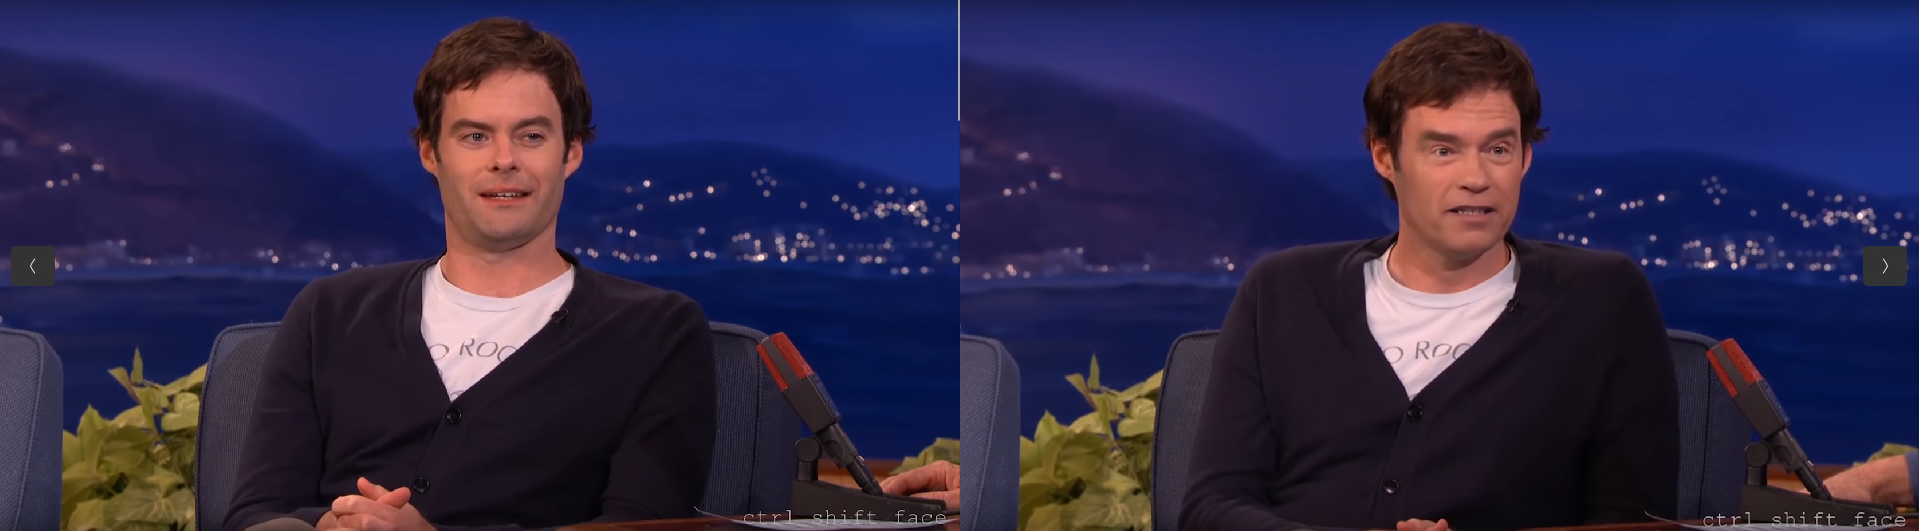
\includegraphics[scale=0.289]{figures/bill-arnold}
	\caption{Deepfake of Bill Hader impersonating Arnold Schwarzenegger. Screenshot from~\cite{bill-hader}}\label{fig:bill-hader}
\end{figure}

The proliferation of deepfake technology became initially sparked with the aid of
its software in creating misleading movie star images and videos, before quickly
expanding into different sectors. One of the earliest examples that drew widespread
interest to deepfakes was a video made by an anonymous Reddit user named `deepfakes'
in late 2017~\cite{10.1145/3491102.3517446, 10.1145/3425780}.
This consumer started to publish digitally altered pornographic motion pictures,
realistically swapping the faces of actresses onto the bodies of porn stars.
While these explicit videos were quickly removed, the sudden emergence of this facial
replacement method, quickly caught the media's eye and circulated on various online forums~\cite{albahar2019deepfakes}.
However, it didn't take long for the technology to be applied beyond explicit content.

A notable example that showcased the potential of deepfakes,
and arguably delivered it to mainstream attention, turned into a video of former
U.S. President Barack Obama, released in April 2018 by Buzzfeed and Jordan Peele~\cite{peele,10.1145/3371409}.
The video features a deepfake of Obama announcing matters he by no means clearly
stated, with Peele providing the voiceover. This deepfake video effectively highlighted
the potential misuse of this technology in spreading misinformation and propaganda.

In recent years, the sophistication of deepfake technology has reached an unprecedented level.
An interesting example of this progression can be seen in the creation of `Tom Cruise deepfakes'
that circulated on social media in early 2021~\cite{deeptomcruise-article}. The videos, created by Belgian visual effects
artist Chris Ume in collaboration with actor Miles Fisher, who impersonated Cruise's voice
and mannerisms, were shared on TikTok under the account name
@deeptomcruise\footnote{\url{https://www.tiktok.com/@deeptomcruise}}~\cite{Agarwal_2021_CVPR,belive-or-not}.
These deepfake videos show the synthetic `Tom Cruise' doing various activities --- performing
a magic trick, playing golf, or simply telling a story about Mikhail Gorbachev~\cite{deeptomcruise}.

The `Tom Cruise deepfakes' took the internet by storm due to their uncanny resemblance to the
real actor, in terms of both appearance and behavior. Unlike the early deepfake videos, which
often exhibited glaring imperfections, these deepfakes were so convincing that many viewers
initially believed they were watching the actual Tom Cruise. This level of realism underscored
the strides made in deepfake technology, while simultaneously highlighting the potential
dangers of its misuse.

Driven by advances in machine learning, especially deep learning, deepfake technology has
grown significantly in sophistication and accessibility. The potential applications of
deepfakes range from benign, such as in film production and entertainment, to malicious uses,
including disinformation campaigns, identity theft, and deepfake pornography. As these
applications become more widespread, deepfake technology has raised profound questions and
challenges for society, especially regarding media authenticity, privacy, and cybersecurity.

However, it is not just the creation of deepfakes that has improved; strides have also been made
in detection. There are now more sophisticated, \ac{AI}-powered tools that can analyze videos
and images for signs of manipulation. These tools operate on multiple levels, from detecting
inconsistencies in lighting and shadows to looking for signs of digital artifacts and abnormal
facial movements. But as detection tools become more sophisticated, so too do the techniques
used to create deepfakes. This constantly evolving technological arms race underscores the
critical need for ongoing research and development in deepfake detection.

In response to these challenges, there is an increasing need for robust and reliable
deepfake detection tools. However, despite the flurry of research and development in this
area, a comprehensive understanding and evaluation of the available detection tools remain
elusive. This knowledge gap not only impedes the technological advancements in deepfake
detection but also complicates the task of policy-making and regulation in this sphere.

This thesis is motivated by the need to bridge this gap and advance our understanding of
publicly-available deepfake detection tools. By examining these tools, this study aims to
contribute to the ongoing efforts to mitigate the risks associated with deepfakes and uphold
the integrity of digital media.


\section{Thesis Structure}\label{chapter:structure}
Understanding the structure of this thesis is essential for a thorough understanding of the
research, as it follows a logical and systematic progression. It starts by laying the basic
groundwork, then gradually delves deeper into the specifics of the study, eventually
integrating the findings and projecting forward-looking discussions. Below is a
detailed outline of the thesis structure, which serves as a roadmap for navigating
the document.

This initial chapter lays the foundation for the thesis. It provides an overview of deepfakes,
introduces the topic of deepfake detection, and outlines the significance and timeliness
of the study. It presents the objectives of the research by addressing three research
questions, clearly stating what the study aims to achieve. The scope and limitations are
also discussed here, delineating the boundaries of the research and acknowledging
its constraints. The introduction serves as a guide, setting the reader's expectations
for the rest of the thesis.

The literature review provides a survey of the existing body of knowledge
related to deepfakes and their detection. The section begins with an explanation of the
techniques used to create deepfakes, giving the reader an understanding of the
technology behind them. This section also highlights the ethical and legal concerns
surrounding deepfakes and the countermeasures and detection methods currently in place.
By identifying gaps and shortcomings in the existing literature, this section also
underscores the relevance and value of the present study.

Chapter three, the methodology along with evaluation metrics and datasets
adopted for the study are outlined. The chapter provides information on how
the publicly-available deepfake detection tools were selected for analysis.
It also discusses the evaluation metrics used to test the effectiveness of these
tools and the datasets used for testing. By detailing these elements, the chapter
ensures that the research process is transparent and replicable.

Chapter four offers an analysis of the six deepfake detection tools: three for video
and three for images. These tools were tested using metrics from~\autoref{chapter:methodology},
looking at their functionality, advantages, and drawbacks.

The fifth chapter takes the analysis from theory to practice, exploring real-world instances
where deepfakes and their detection have played a significant role. The case studies
are chosen to represent a variety of scenarios, thereby providing some of the
practical implications and challenges associated with deepfakes and their
detection.

The sixth chapter presents the findings from the evaluation of the selected tools.
It also provides a comparative analysis of the tools, highlighting their relative
strengths and weaknesses. Subsequently, the results of the comparison are described
and discussed. The research questions from~\autoref{sec:objectives} are also answered here.

The final chapter summarizes the findings and discussions from previous chapters and
reflects on their contribution to the field. It also identifies potential directions
for future research, offering suggestions for how the field can continue to evolve
and adapt in response to the dynamic nature of deepfakes. Finally, a conclusion is drawn,
highlighting current deepfake limitations.

\section{Objectives of the Study}\label{sec:objectives}
Deepfakes have been prominently discussed in both scholarly articles and the media~\cite{forbes-2020,guardian-2019}.
Their ability to convincingly deceive an ordinary user is getting better and better.
For effective countermeasures and understanding of future threats, it's important to understand
deepfake detection technologies. Thus, the primary purpose of the thesis is to provide
an exploration of the state of the art in publicly-available deepfake detection tools.
Specifically, the study addresses these \ac{RQ}:

\begin{itemize}
	\item Research Question 1: How accessible and user-friendly are publicly-available
	      deepfake detection tools for individuals who do not have expertise in deepfakes or
	      detectin deepfakes?
	\item Research Question 2: How effective are deefake detection tools, which are selected
	      and analyzed in this research, in identifying forgeries from various deepfake
	      generation tools?
	\item Research Question 3: What are the privacy implications and policies associated with
	      selected deepfake detection tools?
\end{itemize}

To address the first research question, a methodological approach was adopted. The selection
criteria, encompassing factors like accessibility, user-friendliness, and documentation
are explained. These criteria guide the selection of the six tools examined in this study.
Subsequently, the evaluation metrics are established to assess the strengths and shortcomings
of these detection tools. Initially, all tools undergo an evaluation based on the selection
criteria outlined in~\autoref{chapter:methodology}. The assessment considers factors like
the tool's accessibility, and determining if it's open-source or proprietary. The availability
of support and documentation, including installation guides and usage instructions, is also
examined. The presence or absence of source code, difficulty of use, any internet or
specific software and hardware requirements, and whether the tools are free or paid,
are also considered. These evaluations are detailed further in~\autoref{sec:analysis-tools}.

In response to the second research question, the study evaluates the performance of the
selected tools against a range of deepfakes generated through diverse methods. Initially,
each of the six tools undergoes testing to discern if they can detect deepfakes. The video
detection tools are evaluated using 110 videos, comprising 40 deepfake videos from
DeepFaceLab~\cite{perov2021deepfacelab}, 40 from FaceSwap~\cite{faceswap}, 10 deepfake
videos sourced from the FaceForensics++~\cite{roessler2019faceforensicspp} dataset,
and 20 authentic videos from the same dataset. Image detection tools are assessed using a
total of 123 images: 49 deepfakes produced with FaceApp~\cite{faceapp-app},
54 with Stable Diffusion~\cite{stable-diffusion}, and 20 genuine photographs obtained online.
Furthermore, the training models and techniques utilized, the datasets employed for initial tool
testing, and the programming languages and frameworks are also examined to answer this question.

Regarding the third research question, attention is directed towards the privacy measures of the
selected tools, examining the presence of their privacy policies and their user data handling
methods. This involves examining the potential risks and determining if the tool developers
provide Terms of Use and Privacy Policy for their tools' utilization.

The identification and elaboration of these research questions provide a roadmap for the study,
with each one serving as a crucial stepping-stone toward the understanding of the nature of
the selected publicly-available detection tools. The research questions are then answered in~\autoref{chapter:results},
comparing the strengths and limitations of the selected tools.

\section{Scope and Limitations}\label{chapter:scope}
The study of deepfakes and their detection is a broad field, involving a range of complex and
interrelated topics. Therefore, it is essential to define the specific scope and
limitations of this thesis to clarify what it will and will not cover. These boundaries
not only provide clarity but also help ensure that the research is feasible and can delve
into the chosen topics in sufficient depth.

\subsection{Scope of the Study}
The primary focus of this thesis is on the analysis and evaluation of publicly available
deepfake detection tools. It will cover both the technical and societal aspects of these
tools, including their performance, methodologies, implications, and potential areas for
future development. It will also provide an overview of the current state of deepfake
technology, from its historical development to its modern techniques and applications.

The thesis will mainly concentrate on visual deepfakes, encompassing both images and
videos, aiming to offer an understanding of the deepfake environment. The
research will also explore the dual nature of deepfakes, examining their harmless
and harmful applications. This exploration is crucial to understand the
difficulties involved in detecting deepfakes.

\subsection{Limitations of the Study}
Despite its broad scope, the study is subject to several limitations that should be
acknowledged. Firstly, due to the rapid pace of technological advancements in the field
of deep learning and \ac{AI}, the state of the art in deepfake technology and detection tools
can change swiftly. As a result, while the thesis aims to provide an up-to-date overview
of the field, some of the information might become outdated shortly after publication.

Secondly, given the focus on publicly-available tools, this thesis might not capture
the full spectrum of deepfake detection methodologies. Many sophisticated tools and
techniques might be proprietary or classified information, not accessible for public
use or scrutiny. Thus, while this study will provide an overview of the
available tools, it might not cover the absolute cutting edge in deepfake detection.

Thirdly, while the study aims to objectively evaluate the performance of deepfake
detection tools, it's important to note that this evaluation is based on the
available datasets and metrics. Variations in these datasets, such as the quality
and diversity of the deepfakes included, can impact the results. Moreover, no
single evaluation metric or dataset can fully capture the effectiveness of a tool
in all real-world scenarios.

Fourthly, while the study will explore the societal, ethical, and legal implications
of deepfakes and their detection, a full analysis of these complex and
evolving issues is beyond its scope. These aspects will be discussed primarily in
relation to the main focus of the thesis --- deepfake detection tools --- and may not
cover all the potential implications of deepfakes.

Finally, the study is limited by the inherent challenges associated with deepfake
detection. Deepfakes are a result of advanced \ac{AI} and machine learning techniques,
and detecting them is a complex task that is still an area of active research.
Therefore, the study's findings should be viewed in light of these inherent difficulties.

\subsection{Delimitations of the Study}
While limitations are factors that are out of the researcher's control, delimitations
are boundaries set by the researcher. In this study, due to time and resource constraints,
the analysis will be limited to a few publicly-available deepfake detection tools,
rather than a list of all available tools. Similarly, while the study will discuss
a few illustrative examples of deepfake applications and case
studies, it will not provide a comprehensive review of all possible uses or instances
of deepfakes.

By acknowledging these scopes, limitations, and delimitations, this thesis aims to
provide a clear exploration of publicly-available deepfake detection tools while
being transparent about its boundaries and potential areas of uncertainty.

% !TeX root = ../main.tex
% Add the above to each chapter to make compiling the PDF easier in some editors.

\chapter{Literature Review}\label{chapter:literature}
The literature review sheds light on the understanding of deepfakes, their history,
the technology driving them, the publicly available tools that create them, and
the ethical, legal, and societal issues they raise. Additionally, it examines the
countermeasures that have been developed to detect and deter them.

\section{Techniques Used in Deepfakes}\label{chapter:techniques}
Deepfakes are underpinned by significant advancements in artificial intelligence (\ac{AI})
and machine learning (ML), particularly the areas of deep learning and neural
networks. Central to the creation of deepfakes are two techniques:
autoencoders and \ac{GAN}.

\subsection{Autoencoders}
Autoencoders, are a type of neural network used for learning
efficient encodings or representations of input data~\cite{doi:10.1126/science.1127647}.
In 2006, Hinton et al.~\cite{10.1145/3297156.3297210,doi:10.1126/science.1127647}
raised the concept of deep learning. This idea quickly gained significant attention,
making deep learning a primary focus of research worldwide~\cite{simonyan2015deep}.
The structure of autoencoders has two main parts: an encoder, which simplifies an
image into a latent space\footnote{Latent space is a compressed representation of data where essential
	features are captured in lower dimensions~\cite{enwiki:1169655673}}~\cite{latent-space-medium}, and a decoder,
which rebuilds the image using that simplified representation~\cite{latent-space-medium,enwiki:1170192786}. Deepfakes use this
setup with a common encoder that translates a person into this latent space. This simplified
representation captures essential details about their face and body stance. This can subsequently
be decoded using a model specifically trained for the intended target. So, in other words,
during the encoding phase, it extracts facial details from two distinct individuals,
identifying and storing the shared facial characteristics. Subsequently, in the decoding phase,
it presents the information of these two individuals. The encoding of one person can be
swapped with another, enabling the face of one person to be superimposed onto another
in an eerily realistic manner.

\begin{figure}[ht]
	\centering
	
\includegraphics[scale=0.45]{figures/deepfakes_00d}
	\caption{Autoencoders common structure. Figure from~\cite{autoencoders-image-alazucconi}}\label{fig:autoencoders}
\end{figure}

The figure in~\autoref{fig:autoencoders} presents an image going
into an encoder. The outcome is a simplfied version of that face, ofeten called a latent face~\cite{autoencoders-image-alazucconi}.
Depending on the setup, this latent face might not resemble a typical face. However, when it goes
through a decoder, it's turned back into a face.

An example of using autoencoders is Fakeapp, developed by a Reddit user for deepfake generation~\cite{s22124556,fakeapp-app}.
The process requires encoding and decoding pairs to interchange faces between input and
output images. Distinct image datasets train each pair, but the encoder parameters remain
consistent across both networks. Consequently, both encoder pairs utilize the same network. Given
the consistent facial features such as the eyes, nose, and mouth across various images,
this method allows the encoder to easily recognize similarities between two sets of facial images.

\subsection{Generative Adversarial Networks}
In the field of \ac{AI} and \ac{ML}, two primary methods exist: supervised and unsupervised learning.
The former relies on labeled data\footnote{In machine learning, data labeling involves attaching
	meaningful tags to raw data so that models can learn from it~\cite{labeled-data}.}
for predictions, whereas the latter does not. Noteably, each method has its distinct advantages and
nuances~\cite{ibm-machine-learning}.

\textit{Supervised learning} is a machine learning approach which uses labeled datasets to
instruct algorithms in data categorization or predict outcomes. By using labeled inputs and outputs,
the model calculates its precision and refines itself over time~\cite{supervised-unsupervised}.
Supervised learning can be categorized into two data mining tasks: classification and regression.
Classification involves accurately sorting data into specific groups, like distinguishing between
newspapers and magazines. Meanwhile, regression uses algorithms to discern the relationship between
dependent and independent variables~\cite{ibm-machine-learning}.

\textit{Unsupervised learning} applies algorithms to group and analyze unlabeled datasets,
identifying hidden patterns without requiring human guidance~\cite{supervised-unsupervised}.

Among the concepts and techniques used in \ac{ML}, discriminative and generative models stand out
as two widely used approaches~\cite{generative-discriminative}. So a \textit{generative model}
assesses the distribution of a dataset to determine the probability of a specific example. On the
contrary, a \textit{discriminative model} predicts unseen data using conditional probability
and is applicable for both classification and regression tasks~\cite{generative-discriminative2}.

There are two main types of generative models, \ac{GAN}s and \ac{VAE}~\cite{generative-discriminative}. \ac{GAN}s
introduced by Goodfellow et al.~\cite{goodfellow2014generative}, envolve two
competing neural networks: a generator and a discriminator. The generator produces
fake samples and the discriminator distinguishes between the real and fake samples.
Within a given training dataset, this method is adept at producing new data that mirrors the
statistical properties of the training data. For instance, when taught using pictures, a \ac{GAN}
can create new images that look very real and similar to the original pictures~\cite{enwiki:1169846514}.
While \ac{GAN}s were initially introduced as generative models for unsupervised learning,
they have demonstrated utility in semi-supervised~\cite{salimans2016improved},
fully supervised~\cite{pix2pix2017}, and reinforcement learning~\cite{ho2016generative} contexts.

At the heart of \ac{GAN}s lies the principle of `indirect' training via the discriminator.
This iterative process improves the quality of the generated samples over time as
the generator learns to create more realistic fakes to fool the discriminator. This
arms race pushes the boundaries of what \ac{GAN}s can create, contributing to the
production of deepfakes that are increasingly difficult to detect~\cite{brock2019large}.

\textbf{\ac{GAN}s with alternative architectures.} Various variants of \ac{GAN} structures
and associated generative models exits. In the original paper~\cite{goodfellow2014generative},
\ac{GAN}s were designed using \ac{MLP} and \ac{CNN}. Later on, many other generative models and
architectures, as described in~\autoref{tab:gans}, were introduced~\cite{gans-versions}.

\begin{table}[htpb]
	\caption{Some of \ac{GAN}s with alternate architectures~\cite{gans-versions,enwiki:1169846514}}\label{tab:gans}
	\centering
	\small
	\begin{tabularx}{\textwidth}{l X}
		\toprule
		\textbf{Types of \ac{GAN}s}    & \textbf{Description}                                                \\
		\midrule
		Conditional GAN (CGAN)         & If both the generator and discriminator of
		\ac{GAN}s are conditioned on supplementary information, y, the model becomes
		conditional. This additional data, y, might be class labels or data from
		different sources. To condition the model, y is inputted
		into both the discriminator and generator as an extra input
		layer~\cite{mirza2014conditional}.                                                                   \\
		\addlinespace
		Dual GAN (DGAN)                & A version of \ac{GAN}, named DualGAN,
		uses two networks trained concurrently using two sets of unlabeled images.
		One network is designed for image generation, while the other distinguishes
		between generated and actual images. DualGAN effectively learns two image translators,
		making it suitable for diverse image-to-image translation activities~\cite{yi2018dualgan}.           \\
		\addlinespace
		Stack GAN (StackGAN)           & A modified version of \ac{GAN} uses multiple generators
		stacked together to create a more lifelike image. Stacked \ac{GAN}s compose a
		network designed to produce high-quality images~\cite{zhang2017stackgan}.                            \\
		\addlinespace
		Cycle GAN (CycleGAN)           & CycleGAN is a method for automatically converting
		images from one domain to another, without the need for paired data samples~\cite{zhu2020unpaired}.  \\
		\addlinespace
		Superresolution GAN (SRGAN)    & A \ac{GAN} designed to transform low-resolution images into
		high-resolution outputs. Super-resolution \ac{GAN}s use a combination of deep networks
		and adversarial networks to enhance the clarity of the input data~\cite{ledig2017photorealistic}.    \\
		\addlinespace
		Deep convolutional GAN (DCGAN) & A \ac{GAN} that employs deep convolutional networks
		for both the generator and discriminator. This \ac{GAN} relies solely on convolution
		and deconvolution layers. Studies suggest that images produced by the DCGAN
		architecture exhibit notably reduced noise~\cite{radford2016unsupervised}.                           \\
		\addlinespace
		Self-attention GAN (SAGAN)     & The SAGAN facilitates attention-based, extended-range
		dependency modeling in image creation. In SAGAN, cues from all feature areas can
		be utilized to produce details. Additionally, the discriminator ensures that intricate
		details in separate parts of the image are consistent with each other~\cite{zhang2019selfattention}. \\
		\bottomrule
	\end{tabularx}
\end{table}

\subsection{Variational Autoencoders}
Recent developments have seen the rise of \ac{VAE} and their use in deepfake
generation~\cite{kingma2022autoencoding}. Unlike traditional autoencoders, \ac{VAE}s introduce
a probabilistic spin to the encoding and decoding processes. The encoder, often
designed using neural networks like the feedforward convolutional network,
learns to encode input data into a latent space. The decoder, also based
on a convolutional neural network, then reconstructs the original input
from this latent space~\cite{vae-gan}. This allows for the
generation of new faces by sampling from the learned distribution, enhancing the
ability of the deepfake technology to generate entirely new, but convincing, faces.

While both \ac{VAE}s and \ac{GAN}s are used for image generation, their methodologies differ.
One primary distinction is their training approach. \ac{VAE}s use an unsupervised learning
technique, aiming to maximize the likelihood of the generated output relative to the
input and compress the input into a latent space. Conversely, \ac{GAN}s are trained
in a supervised learning technique, striving for equilibrium between the generator
and discriminator, where the former seeks to fool the latter. Furthermore, \ac{VAE}s
often have a more straightforward training process compared to \ac{GAN}s because they
don't require tight coordination between their components. Additionally, due to their
advanced capabilities, \ac{GAN}s are often used for demanding tasks such as
super-resolution and image-to-image translation. On the other hand, \ac{VAE}s are
predominantly used for image denoising and generation~\cite{vae-gan}.

\section{Publicly Available Deepfake Generation Tools}\label{chapter:publicly}
As deepfake technology has evolved, so too has the ease of access to this technology.
There are now several deepfake generation tools that are freely available and relatively
easy to use, drastically lowering the bar for entry into the world of deepfakes.

\subsection{DeepFaceLab}\label{sec:deepfacelab}
DeepFaceLab\footnote{\url{https://github.com/iperov/DeepFaceLab}}~\cite{perov2021deepfacelab,10.1117/12.2631297}
was developed to address the challenges and inefficiencies typically
observed in deepfake generation models~\cite{s22124556}. This refined framework,
facilitates face-swapping~\cite{perov2021deepfacelab}. The architecture incorporates
an `encoder' and `destination decoder', separated by an `inter' layer, and
concludes with an `alignment' layer. To extract features, it uses the 2DFAN~\cite{Bulat_2017}
heat map-based facial landmark algorithm, and for face segmentation,
it utilizes the TernausNet~\cite{iglovikov2018ternausnet}.

\begin{figure}[htpb]
	\centering
	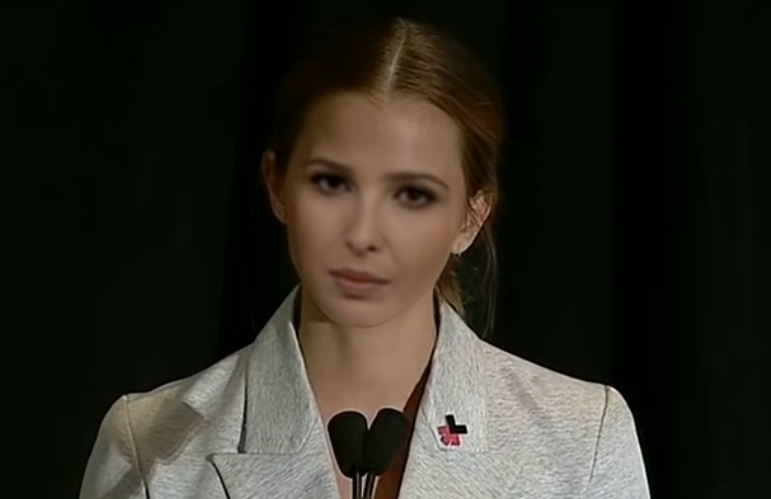
\includegraphics[scale=0.36]{figures/ivanka-deepfacelab}
	\caption{Deepfake of Ivanka Trump impersonating Emma Watson. Screenshot
		from our own generated deepfake video dataset with DeepFaceLab.}
\end{figure}

Known for offering greater functionality and control over the deepfake creation
process, DeepFaceLab has been used in several high-profile deepfake videos.
Its sophisticated technology combines the power of \ac{GAN}s and autoencoders,
leading to highly realistic face swaps in videos. DeepFaceLab offers tools
for every step of the deepfake creation process, including face extraction,
training, and video creation. This comprehensive suite of tools, combined
with its high-quality results, make it a popular choice among deepfake creators.

\subsection{FaceSwap}\label{sec:faceswap}
Faceswap typically refers to the replacement of one person's face with another's
in images or videos. In this context, it signifies a specific technique
implemented in~\cite{faceswap}. The method operates frame-by-frame for both
source and target videos until one ends. Within each image, distinct
facial landmarks such as face contour, eyes, mouth, and other distinguishing
facial features are identified. Utilizing the landmarks from the source image,
a 3D representation of the source actor's face is constructed. This is then
adjusted to align with the target actor's facial landmarks and integrated
into the target image. After processing each frame, the result is a video
wherein the target actor's face is substituted by the source
actor's~\cite{deepfakes-thesis,9897972,Korshunova_2017_ICCV}.

\begin{figure}[htpb]
	\centering
	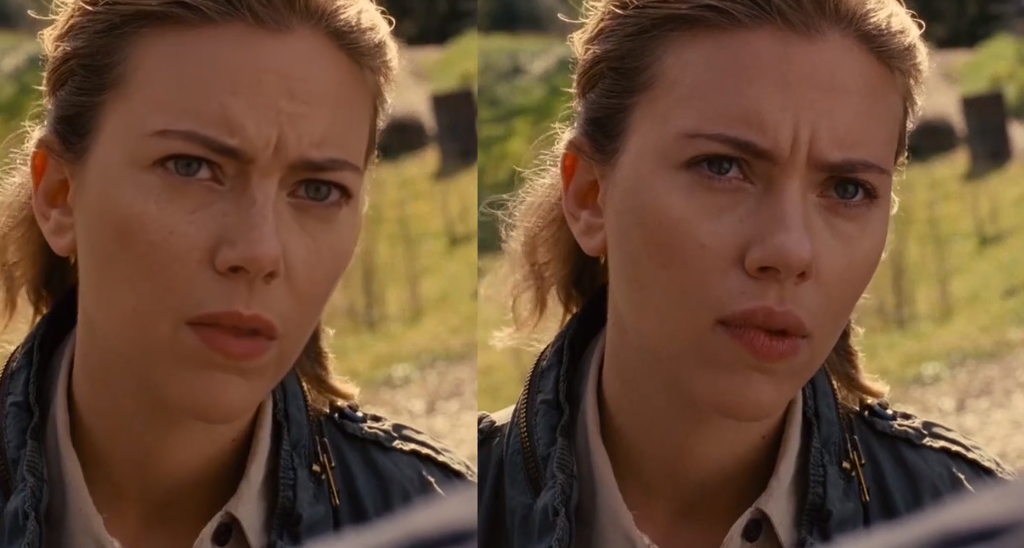
\includegraphics[scale=0.32]{figures/emma-stone-faceswap}
	\caption{Deepfake of Emma Stone impersonating Scarlett Johansson using
		Faceswap. Screenshot from~\cite{emma-stone-faceswap}.}
\end{figure}

This community-based deepfake tool stands out with its open-source nature,
providing the user with a choice of multiple \ac{AI} models. It caters to
varying levels of experience and computing resources, making it accessible
to a wide range of users. Besides its technical merits,
FaceSwap\footnote{\url{https://faceswap.dev}} emphasizes the ethical use
of deepfake technology, warning against non-consensual use of a person's
likeness. It is more than just a tool; it's a community where people can
learn, discuss, and share knowledge about deepfakes.

\subsection{Stable Diffuison}\label{sec:stable-diffusion}
Recently, image synthesis methods using diffusion models centered on denoising
techniques~\cite{ho2020denoising} have gained popularity because of their impressive
outcomes in generating artificial artwork~\cite{10.1145/3588015.3589842}.
Notably, latent diffusion models like \ac{SD}~\cite{rombach2022highresolution}
empower individuals to produce images from textual prompts effectively,
even using personal computers.

Introduced in 2022~\cite{rombach2022highresolution}, Stable Diffusion is a deep learning
model utilizing diffusion methods, primarily for generating intricate images based
on textual inputs. It also has applications in inpainting\footnote{Inpainting refers
	to the restoration technique where absent or damaged sections of an artwork are
	replenished to display a complete image~\cite{enwiki:1164523541}.},
outpainting, and facilitating image-to-image conversions guided by a text
prompt~\cite{sd-hugging-face}. The model was a collaborative effort from the CompVis Group
at Ludwig Maximilian University of Munich~\cite{enwiki:1169859793}, Runway,
Stability AI\footnote{\url{https://stability.ai/stablediffusion}}, and
several non-profit organizations~\cite{sifted-2020,sd-lmu,stabilityai}.

As a latent diffusion model, Stable Diffusion is a type of deep generative neural network.
Its code and model parameters are publicly available~\cite{sd-github}, and it's
compatible with consumer-grade hardware having a GPU with a minimum of
8 GB~\cite{enwiki:1169859793}. This is in contrast to previous models like DALL-E~\cite{dall-e}
and Midjourney~\cite{midjourney}, which were restricted to cloud-based access~\cite{enwiki:1169859793,sd-theverge}.

\begin{figure}[htpb]
	\centering
	
\includegraphics[width=0.59\columnwidth]{figures/justion-trudeau-stable-diff}
	\caption{Deepfake of Justin Trudeau created with Stable Diffusion.
		Screenshot from our own generated deepfake video dataset with Stable Diffuison.}
\end{figure}

Stable Diffusion models utilize a diffusion process to generate realistic synthetic
images from a simple Gaussian noise, achieving impressive results in the generation of
deepfake images~\cite{wu2022unifying}. One of the benefits of diffusion models
is that they can capture complex, multi-modal distributions in a way that
other generative models may struggle with. This makes them particularly
well-suited for tasks like deepfake generation, where capturing the
detailed, multi-modal distribution of human faces is essential.

\subsection{Neural Textures}
Introduced by Thies et al.~\cite{thies2019deferred}, Neural Textures represent
a method for the storage, transmission, and rendering of learned
neural representations in the context of computer graphics.
By rendering with learned features instead of geometric detail, Neural
Textures allow for more efficient representations, enabling high-quality,
photorealistic image synthesis and editing. Specifically, in the realm of
deepfakes, Neural Textures, as shown in~\autoref{fig:neural_textures}, can be trained to synthesize person-specific
details, resulting in high-quality face swaps or manipulation of facial
expressions in videos.

\begin{figure}[htpb]
	\centering
	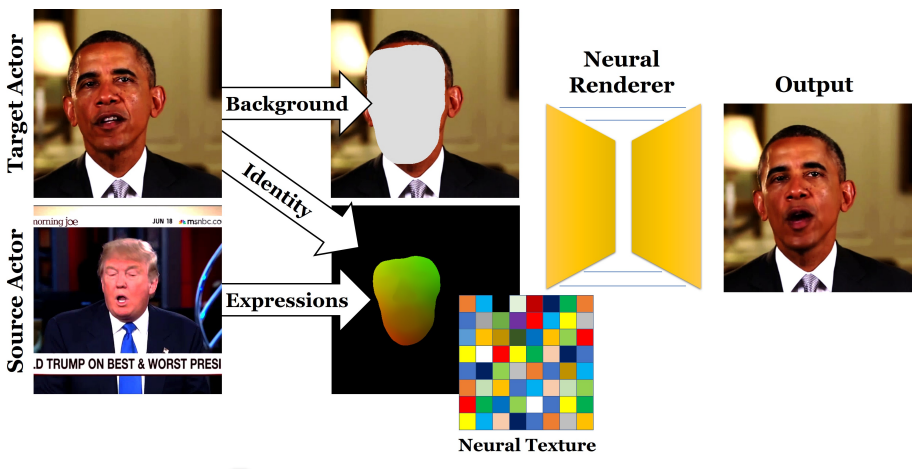
\includegraphics[scale=0.55]{figures/neural_textures}
	\caption{The reenactment synthesis process uses expression transfer
		to generate a UV map of the target actor that reflects the source
		actor's expression. This map, along with a background image, is
		processed by a neural renderer to create the final reenactment.
		Expression alteration is achieved by training a unique neural
		texture and renderer for the target actor, resulting in a
		manipulated video as shown in the image from~\cite{thies2019deferred}.}\label{fig:neural_textures}
\end{figure}

Neural textures utilize a UV-map\footnote{UV mapping involves projecting a 3D model's surface
	onto a 2D plane for the purpose of texture mapping~\cite{enwiki:1169139226}.}
connecting elements in the texture map to object points, allowing the creation of a
viewpoint-specific texture. Integrating this into a trained deferred neural renderer
produces an image from the designated viewpoint, as illustrated in~\autoref{fig:neural-textures2}.
While neural textures have various uses, Thies et al.~\cite{thies2019deferred} highlight
facial video manipulation. \autoref{fig:neural_textures} demonstrates this application,
paralleling the Face2Face~\cite{thies2020face2face} method. Training videos establish a
3D face model of the target actor. Additionally, a unique neural texture and deferred neural
renderer are crafted for this actor. Leveraging the Face2Face expression transfer
technique, a UV-map from the target video is adjusted to mirror the source actor's
expressions. With this UV-map, the neural texture, and renderer, the manipulated video emerges.

\begin{figure}[htpb]
	\centering
	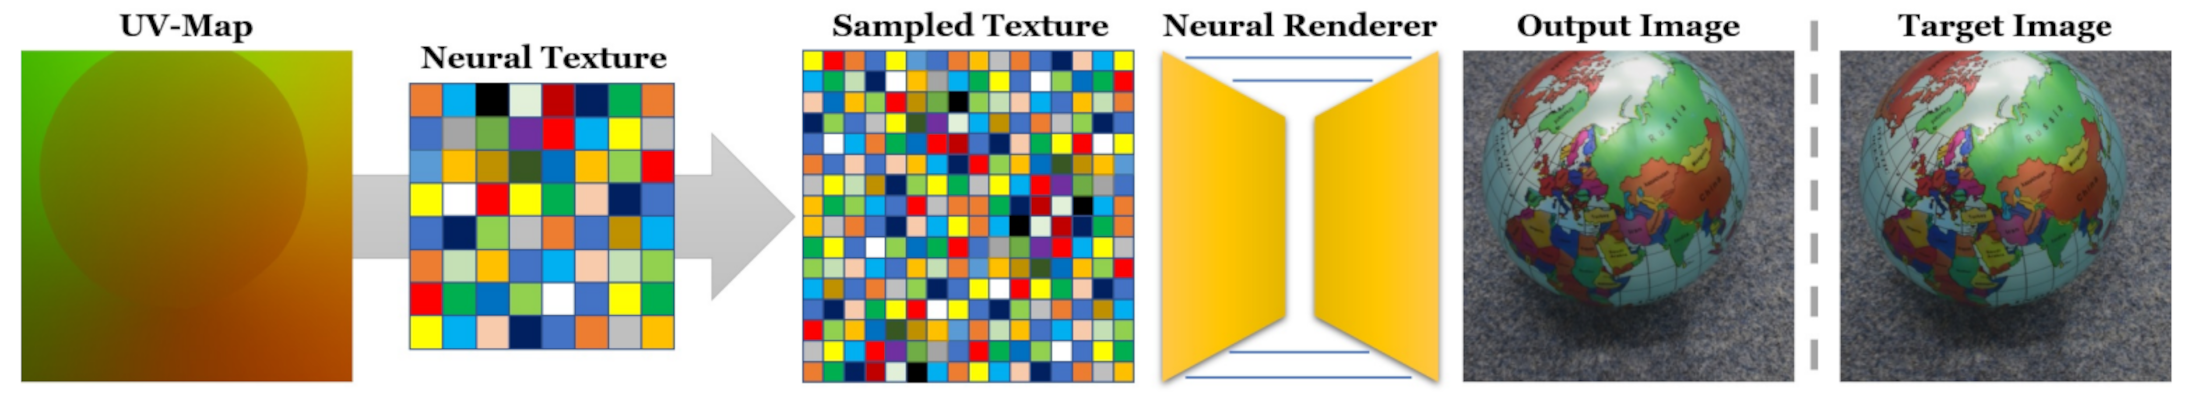
\includegraphics[scale=0.25]{figures/neural_textures2}
	\caption{Overview of neural rendering pipeline~\cite{thies2019deferred}.}\label{fig:neural-textures2}
\end{figure}

\subsection{FaceApp}\label{sec:faceapp}
While not a deepfake tool in the traditional sense,
FaceApp\footnote{\url{https://www.faceapp.com/}} has gained popularity due
to its ability to transform photos of faces in various ways, such as aging,
de-aging, gender swapping, and adding smiles~\cite{wirth2023interface}.
Introduced in 2017~\cite{wirth2023interface} by the Russian startup Wireless Lab, now known
as FaceApp Technology Limited, the FaceApp software enables users to undertake
detailed photo and video modifications. These include aging or rejuvenating facial
appearances, merging two faces, incorporating intricate facial expressions like smiles,
and utilizing the debated `gender swap' function.

\begin{figure}[htpb]
	\centering
	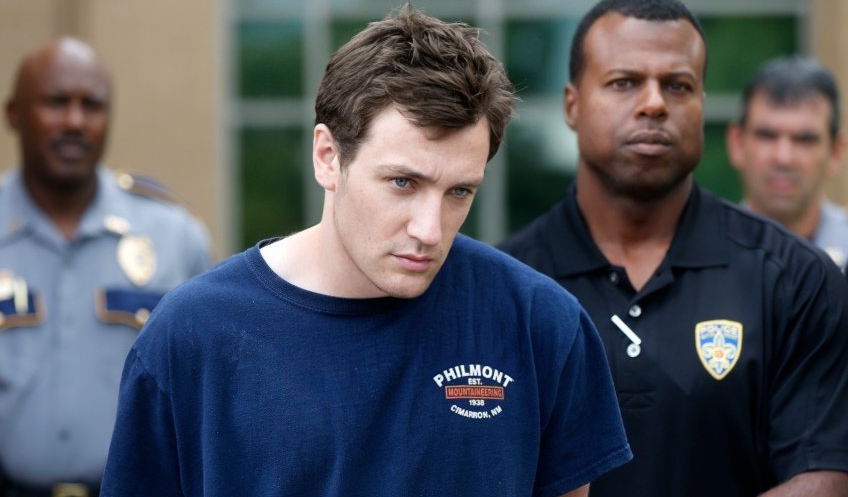
\includegraphics[width=0.61\columnwidth]{figures/faceapp}
	\caption{Deepfake created with FaceApp. Screenshot from our own generated deepfake image
		dataset with FaceApp.}
\end{figure}

The tool leverages neural network technology for its transformations, leading to surprisingly
realistic results that have significantly contributed to the broader conversation
around the manipulation of digital imagery~\cite{faceapp}. FaceApp has
been both praised for its technological achievements and criticized for
its potential privacy and consent issues~\cite{warzel2019faceapp}, reflecting the wider debates
surrounding the ethical implications of deepfake technology.

In essence, FaceApp's image processing capabilities go beyond just simple pixel-altering
image filters. Initially, each image is transformed into a multi-dimensional vector which
might subsequently serve as a foundation for modification --- essentially a reshuffling
of the neural weights in the network~\cite{faceapp-article1}. When using FaceApp's tools,
the \ac{CNN} superimposes specific features onto the chosen portrait or selfie, features
that have been extracted from its training dataset. Thanks to sophisticated image recognition
techniques, precise automatic feature adjustments are made, resulting in notably photorealistic
effects. Intriguingly, while fundamentally transforming the image, FaceApp preserves
unique facial features~\cite{faceapp-medium}. This allows users to perceive alterations, like aging or
rejuvenation, as authentic modifications to their own faces~\cite{wirth2023interface,faceapp-article2}.

\section{Ethical and Legal Concerns}\label{chapter:legal}
The rise of deepfakes has brought with it a number of ethical and legal concerns.
At the forefront is the issue of consent, as deepfakes often involve the
use of a person's identity without their permission. This has been
particularly common in the creation of deepfake pornography, leading
to significant harm and distress for the individuals involved~\cite{chesney2019deep}.

There are also concerns about the potential misuse of deepfakes in spreading
disinformation and propaganda. Deepfakes could be used to manipulate public
opinion, interfere in elections, or even incite violence~\cite{deepfakes-business-insider,partnershiponai}.
The realistic nature of deepfakes makes it difficult for the average viewer
to distinguish truth from fake, further exacerbating these risks.

In journalism, the rise of deepfakes presents both a significant
challenge and an ethical dilemma. Journalists must not only cope with
the complex task of verifying the authenticity of deepfake content
but also think about the ethical implications of using \ac{AI}-generated
content in their reporting. Misuse of deepfakes could lead to the spread of
false information, shaking people's faith in the media~\cite{doi:10.1177/2056305120903408}.

Furthermore, the use of deepfake technology can be used to fabricate evidence in
legal cases, potentially leading to miscarriages of justice. As deepfakes become
increasingly indistinguishable from real videos, the legal system will need to
find ways to authenticate digital evidence and mitigate the risk of deepfake-generated
evidence~\cite{chesney2019deep}.

The business sector is not immune to the impact of deepfakes either. Businesses
could fall victim to deepfake scams, in which \ac{AI}-generated audio or video
is used to impersonate a company employee or other authority figure.
These scams could lead to significant financial losses or damage to a
company's reputation~\cite{MUSTAK2023113368}.

Lastly, in deepfake detection, a crucial concern is the issue of
false positives and negatives. A false positive, where a real video is wrongly
flagged as a deepfake, could have serious consequences, such as the unnecessary
spread of panic or unwarranted damage to an individual's reputation. On the
other hand, a false negative, where a deepfake is not detected and is thus
taken as genuine, can lead to the propagation of disinformation or fraud.
These challenges underscore the need for highly careful deepfake detection methods~\cite{roessler2019faceforensicspp}.

\section{Existing Countermeasures and Detection Methods}\label{chapter:countermeasures}
The rise of deepfakes demand effective countermeasures and detection methods
to ensure information integrity and maintain public trust
in digital content. As deepfake generation techniques have become more advanced,
detection approaches have adapted accordingly. Many of these
approaches use machine learning, particularly deep learning techniques,
leveraging similar technologies that power deepfakes to combat them.

The general idea of deepfake detection is based on identifying inconsistencies
or anomalies that typically arise during the process of creating deepfakes. These
can be artifacts left by the specific algorithm used, unusual patterns in the
distribution of the pixel values, or unnatural physical characteristics
such as inconsistent lighting or improper blinking patterns~\cite{Agarwal_2019_CVPR_Workshops}.

One approach to detect deepfakes is frequency-based analysis, where the focus is
on the differences in frequency patterns between original and deepfaked videos.
These methods, like the one proposed by Durall et al.~\cite{durall2020unmasking},
take advantage of the fact that, deepfake generation algorithms usually function in
spatial domain~\cite{spatial-domain}. As a result, they may produce distinct inconsistencies
within the frequency domain.

Another widely used approach is the \ac{CNN} based detection. This type of deep
learning model has shown excellent performance in various image and video
processing tasks due to its ability to learn hierarchical patterns in the data.
For deepfake detection, \ac{CNN}s can be trained to learn the differences between
real and fake images or videos, thus distinguishing deepfakes from the original
media~\cite{nguyen2018capsuleforensics}.

Another promising approach is the use of autoencoders for deepfake detection.
Autoencoders are a type of neural network that are trained to reconstruct
their input data. By training an autoencoder on a large amount of real face
data, it can learn to recreate real faces very well, but struggle to recreate
deepfakes, allowing the detection of deepfakes based on the reconstruction
error~\cite{cozzolino2017recasting}.

Recent advancements have led to the development of deepfake detection techniques
that analyze physiological signals. For instance, Li et al.~\cite{li2018ictu}
developed a method based on the observation that real videos contain physiological
signals that are driven by blood flow, such as heart rate. These signals, they
found, are not well preserved in synthetically generated data and thus provide
a new cue for deepfake detection.

It's important to note, however, that as deepfake generation techniques
continue to evolve, the effectiveness of these detection methods can diminish.
The constant race between deepfake creation and detection presents ongoing
challenges for researchers and developers in maintaining the efficacy of these
countermeasures.
% !TeX root = ../main.tex
% Add the above to each chapter to make compiling the PDF easier in some editors.

\chapter{Methodology}\label{chapter:methodology}

\section{Research Design}\label{chapter:research}
\section{Selection Criteria for Publicly-Available Tools}\label{chapter:selection}
\section{Evaluation Metrics}\label{chapter:evaluation}
\section{Datasets}\label{chapter:data}
\section{Overview of Selected Publicly-Available Deepfake Tools}
% !TeX root = ../main.tex
% Add the above to each chapter to make compiling the PDF easier in some editors.

\chapter{Analysis of Publicly-Available Deepfake Tools}\label{chapter:tools}

\section{Sensity}\label{chapter:sensity}
\section{FaceForensics++}\label{chapter:faceforensics}
\section{FaceSwap}\label{chapter:faceswap}
\section{XceptionNet}\label{chapter:xceptionnet}
\section{Comparative Analysis}\label{chapter:analysis} 
% !TeX root = ../main.tex
% Add the above to each chapter to make compiling the PDF easier in some editors.

\chapter{Case Studies}\label{chapter:applications}
With the bond of art and technology, deepfakes are slowly redefining the state of
entertainment. Their ability to transform audio and visuals offers creators better
possibilities to create new types of content. From refining the quality of amateur
videos to colorizing black-and-white movies, deepfakes are reshaping the entertainment
and art industries.

However, as explored in this research, the rise of deepfakes also underscores the pressing
need for effective detection mechanisms. The tools discussed in this thesis have direct
implications for the case studies presented here, as they offer potential solutions
to the challenges posed by deepfakes in various sectors.


\section{Entertainment and Art}
Deepfakes are popular in many creative areas. For example, rapper Kendrick Lamar
used deepfake in the 2022 music video to take on the looks of celebrities. In the
renewed Star Wars series, deepfake technology was used to resurrect characters like
Princess Leia and Moff Tarkin, despite the original actors having passed away~\cite{motion-analysis}.

The emergence of deepfake detection tools can play an important role in ensuring the
integrity of content in the entertainment industry. For instance, tools that can swiftly
and accurately detect manipulated content can help filmmakers and artists ensure that
their work remains authentic and free from unauthorized alterations.

The real question is: Is deepfake technology a blessing or a curse for talent?
An actor can feature in global commercials or websites
without constant traveling or learning new languages. For instance, Synthesia\footnote{\url{https://www.synthesia.io/}}
did this with two commercials starring rapper Snoop Dogg. Instead of reshooting for a
rebranded commercial, they altered Snoop Dogg's mouth movements to match the new brand
name using deepfakes~\cite{wipo-magazine}.

One of the positive implications of deepfakes in the Arts industry is, for example, the Salvador
Dalí Museum introduced \textit{Dalí Lives}, a digital revival of the deceased artist
Salvador Dalí using deepfakes~\cite{salvador-dali, salvador-dali2}.
This allows visitors to interact with the artist, hearing tales from his life, and
even taking selfies. The Museum used an encoder-decoder deepfake technique, training encoders on Dalí's
images and footage. An actor resembling Dalí was then mapped with Dalí's features using
decoders (\autoref{dali-youtube}).

\begin{figure}[ht]
	\centering
	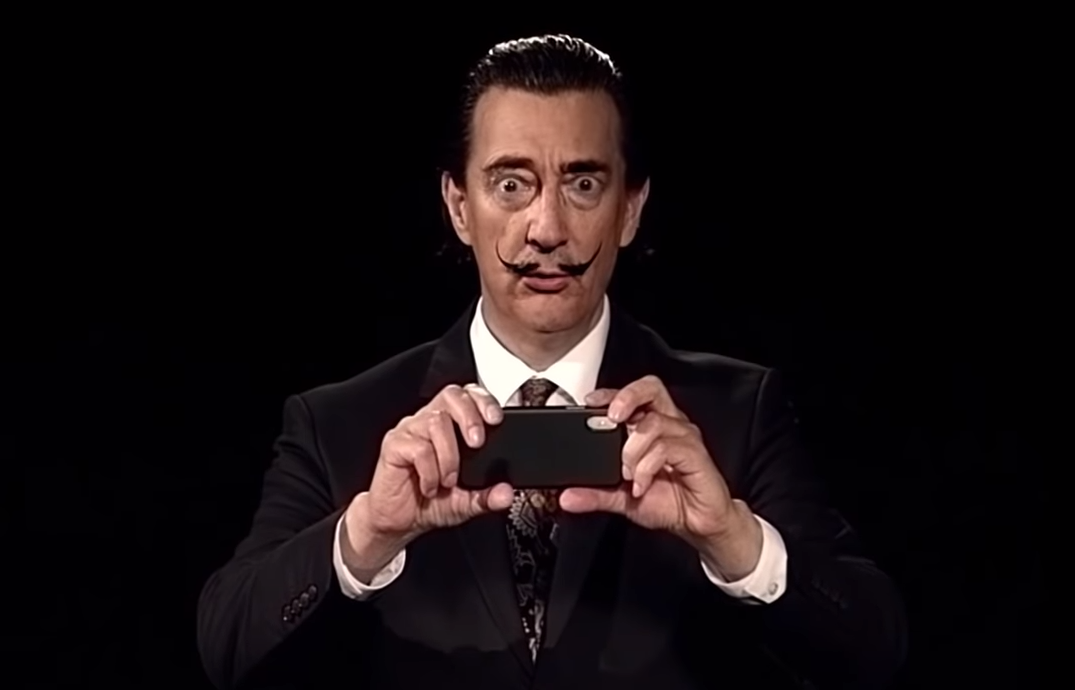
\includegraphics[width=0.61\columnwidth]{figures/dali}
	\caption{Screenshot taken from Dalí Lives~\cite{salvador-dali-youtube}.}\label{dali-youtube}
\end{figure}

Deepfakes, while being helpful and revolutionary, have notable weaknesses and can pose serious
threats. They have been misused for creating fake celebrity videos, committing fraud, and manipulating
political content, leading California to ban making political deepfakes during election
season in 2019~\cite{salvador-dali,california}. Such instances underscore the pressing need for
robust deepfake detection tools.


\section{Politics and Media}
With the rise of deepfakes in politics, the demand for effective detection tools
has also surged. Given the potential for deepfakes to influence public opinion,
especially during critical events like elections, there's an urgent need for tools
that can quickly and accurately identify manipulated content.

On the positive side of this context,
some political figures have used deepfakes in their campaigns for creative advertisements.
For instance, during the 2020 Delhi Legislative Assembly election in India, a deepfake video
of the president of India's \ac{BJP} party, Manoj Tiwari, spread on WhatsApp, as reported
by Vice~\cite{vice}. In this first-ot-its-kind campaign use, the original video of Tiwari speaking
English was changed to appear as if he spoke in Haryanvi, a Hindi dialect, targeting specific
voters. The \ac{BJP} collaborated with The Ideaz Factory to produce such deepfakes, aiming to
reach India's diverse linguistic audience. This particular deepfake reached reportedly 15 million
people across WhatsApp groups~\cite{india}.

Another case from politics involves a deepfake video created by Jordan Peele, where he
impersonated former U.S. President Barack Obama~\cite{peele,10.1145/3371409}. The video, widely
circulated on YouTube, depicted Obama making unexpected remarks, but was later revealed to be
manipulated with Peele's voice. When this video was analyzed using the Deepware deepfake
detection tool, it identified the content as a deepfake with a 93\% probability. This instance
highlights the importance of detection tools like Deepware in monitoring and verifying
political content.

\begin{figure}[ht]
	\centering
	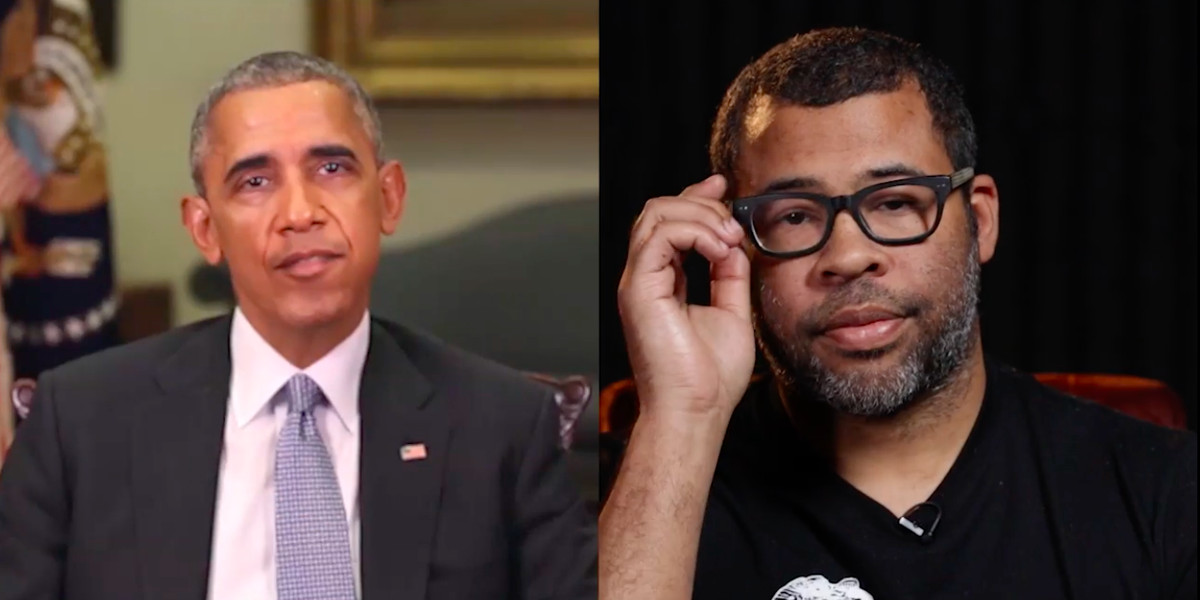
\includegraphics[width=0.8\columnwidth]{figures/obama}
	\caption{Screenshot taken from BuzzFeedVideo~\cite{peele}.}\label{obama-youtube}
\end{figure}

The risk of spreading misinformation in politics is high. There have been past
occurrences where fake videos were used to damage the reputation of political individuals.
Regulating political deepfakes is complex. While potential laws could aim to ban manipulated
content of politicians, they'd need exceptions to safeguard artistic and satirical content,
making implementation of those laws challenging due to the nature of satire and art~\cite{politics,vanity-fair}.
Promising solutions are emerging in the tech industry, as tech giants like Adobe and Microsoft,
alongside startups like Truepic\footnote{\url{https://truepic.com/}}, are developing tools for
authenticity verification.
% !TeX root = ../main.tex
% Add the above to each chapter to make compiling the PDF easier in some editors.

\chapter{Results}\label{chapter:results}
In this chapter, the results of the in \autoref{sec:analysis-tools} computed experinments are
presented. As previously described, three different video and image detection tools were used
to detect deepfakes. Calculations for the video detection tools were based on the
FaceForensics++ dataset, along with deepfake videos produced by DeepFaceLab and FaceSwap.
Image detection tools were evaluated using images created by FaceApp and Stable Diffusion,
as well as 20 authentic images.

\section{Comparative Results of tools}

\begin{figure}[htbp]
	\centering
	\begin{subfigure}{0.48\textwidth}
		\centering
		\begin{tikzpicture}
			\begin{axis}[
					ybar,
					bar width=5mm,
					width=7cm,
					height=7cm,
					enlarge x limits=0.2,
					legend style={at={(0.5,-0.2)},
							anchor=north,legend columns=-1},
					ylabel={Avg. Time in seconds},
					ylabel shift=-3pt,
					symbolic x coords={Deepware, Seferbekov, NtechLab},
					xtick={Deepware, Seferbekov, NtechLab},
					ytick={20,60,120,180,300,400,480},
					ymin=0,
					ymax=540,
					ymajorgrids=true,
					nodes near coords,
					every node near coord/.append style={font = {\fontsize{9 pt}{12 pt}\selectfont},color=black},
				]
				\addplot [orange,fill=orange!30,bar shift=-0.3mm] coordinates {(Deepware,21.5)};
				\addplot [blue,fill=blue!30] coordinates {(Seferbekov,67.25)};
				\addplot [red,fill=red!30, bar shift=0.3mm] coordinates {(NtechLab,480)};
			\end{axis}
		\end{tikzpicture}
		\caption{Video detection}
	\end{subfigure}
	\hfill
	\begin{subfigure}{0.48\textwidth}
		\centering
		\begin{tikzpicture}
			\begin{axis}[
					ybar,
					bar width=5mm,
					width=7cm,
					height=7cm,
					enlarge x limits=0.2,
					legend style={at={(0.5,-0.2)},
							anchor=north,legend columns=-1},
					ylabel={Avg. Time in seconds},
					ylabel shift=-6pt,
					symbolic x coords={Facetorch, Illuminarty, AI or Not},
					xtick={Facetorch, Illuminarty, AI or Not},
					ytick={0,3,6,9,12,15},
					ymin=0,
					ymax=17,
					ymajorgrids=true,
					nodes near coords,
					every node near coord/.append style={font = {\fontsize{9 pt}{12 pt}\selectfont},color=black},
				]
				\addplot [orange,fill=orange!30,bar shift=-0.3mm] coordinates {(Facetorch,13.5)};
				\addplot [blue,fill=blue!30] coordinates {(Illuminarty,3.9)};
				\addplot [red,fill=red!30, bar shift=0.3mm] coordinates {(AI or Not,3.2)};
			\end{axis}
		\end{tikzpicture}
		\caption{Image detection}
	\end{subfigure}
    \caption{Comparison of the Processing Time of detection tools from~\autoref{sec:analysis-tools}}\label{fig:processing-time}
\end{figure}

From~\autoref{fig:processing-time}, it's evident that image detection tools process data faster
than the video detection tools. This discrepancy is due to the nature of the tools:
image detection tools only process a single image (frame), whereas video detection tools may 
need to break a video into numerous frames and analyze each one separately, which is considerably
more time-consuming. Additionally, among the video detection tools, NtechLab's tool was slower than 
both Deepware and Seferbekov's tool. This might be because of the detection techniques they used.

The duration a tool takes to process data is tied to the size of the input. For instance, 
Seferbekov's tool, when handling a video under 10MB, averaged a processing time of 20 seconds. However,
when confronted with a video exceeding 70MB, the time nearly tripled to almost a minute. 
The size-to-time relationship is consistent across all tools, meaning the larger the size of the
input, the longer it's going to take the tool to process it.

A comparison of assessed metrics for video detection tools is displayed in~\autoref{fig:comparison_video}.
The comparison of which tool performed better is interesting. As we know, accuracy and precision 
are defined as follows: Accuracy measures the fraction of all instances that are correctly 
identified and precision measures the fraction of instances that were correctly predicted as 
positive out of all predicted positives. So precision is especially important when the number
of false positives is high. In both of these cases NtechLab performed than the other two 
tools. This is due to the fact that NtechLab could detect more deepfakes.

Recall, also known as sensitivity, measures the proportion of actual positives that were 
correctly identified. It is crucial when the cost of missing a pisitive instance is high.
And F-1 Score is a metric providing a balance between preicision and recall, offering a more 
comprehensive view of the performance. While NtechLab had higher accuracy and precision, 
Deepware and Seferbekov's tool have caught up in terms of Recall and F1-Score. This suggests that
Deepware and Seferbekov's tool were more effective at correctly identifying true positive cases.

When it comes to image detection tools in~\autoref{fig:comparison_image}, AI or Not and 
Illuminarty outperformed Facetorch. One possible reason could be that AI or Not and 
Illuminarty are supported by companies and communities, receiving consisten updates. 
On the other hand, Facetorch is an open-source project. It hasn't had any updates 
since March 2023, which might make it less equipped to handle newer deepfake generation
techniques.

\begin{figure}[htbp]
	\centering
	\begin{subfigure}{0.48\textwidth}
		\centering
		\begin{tikzpicture}
			\begin{axis}[
					ybar,
					bar width=5mm,
					width=7.2cm,
					height=8cm,
					enlarge x limits=0.2,
					legend style={at={(0.5,-0.2)},
							anchor=north,legend columns=-1},
					ylabel={Percentage},
					ylabel shift=-6pt,
					symbolic x coords={Deepware, Seferbekov, NtechLab},
					xtick={Deepware, Seferbekov, NtechLab},
					ytick={0,20,40,60,80,100},
					ymin=0,
					ymax=110,
					ymajorgrids=true,
					nodes near coords,
					every node near coord/.append style={font = {\fontsize{9 pt}{12 pt}\selectfont},color=black},
				]
				\addplot [orange,fill=orange!30,bar shift=-0.3mm] coordinates {(Deepware,88.18)};
				\addplot [blue,fill=blue!30] coordinates {(Seferbekov,88.18)};
				\addplot [red,fill=red!30, bar shift=0.3mm] coordinates {(NtechLab,98)};
			\end{axis}
		\end{tikzpicture}
		\caption{Detection accuracy}
	\end{subfigure}
	\hfill
	\begin{subfigure}{0.48\textwidth}
		\centering
		\begin{tikzpicture}
			\begin{axis}[
					ybar,
					bar width=5mm,
					width=7.2cm,
					height=8cm,
					enlarge x limits=0.2,
					legend style={at={(0.5,-0.2)},
							anchor=north,legend columns=-1},
					ylabel={Percentage},
					ylabel shift=-6pt,
					symbolic x coords={Deepware, Seferbekov, NtechLab},
					xtick={Deepware, Seferbekov, NtechLab},
					ytick={0,20,40,60,80,100},
					ymin=0,
					ymax=110,
					ymajorgrids=true,
					nodes near coords,
					every node near coord/.append style={font = {\fontsize{9 pt}{12 pt}\selectfont},color=black},
				]
				\addplot [orange,fill=orange!30,bar shift=-0.3mm] coordinates {(Deepware,91.40)};
				\addplot [blue,fill=blue!30] coordinates {(Seferbekov,97.53)};
				\addplot [red,fill=red!30, bar shift=0.3mm] coordinates {(NtechLab,98.75)};
			\end{axis}
		\end{tikzpicture}
		\caption{Precision}
	\end{subfigure}

    \vspace{0.5cm}

    \begin{subfigure}{0.48\textwidth}
		\centering
		\begin{tikzpicture}
			\begin{axis}[
					ybar,
					bar width=5mm,
					width=7.2cm,
					height=8cm,
					enlarge x limits=0.2,
					legend style={at={(0.5,-0.2)},
							anchor=north,legend columns=-1},
					ylabel={Percentage},
					ylabel shift=-6pt,
					symbolic x coords={Deepware, Seferbekov, NtechLab},
					xtick={Deepware, Seferbekov, NtechLab},
					ytick={0,20,40,60,80,100},
					ymin=0,
					ymax=110,
					ymajorgrids=true,
					nodes near coords,
					every node near coord/.append style={font = {\fontsize{9 pt}{12 pt}\selectfont},color=black},
				]
				\addplot [orange,fill=orange!30,bar shift=-0.3mm] coordinates {(Deepware,94.44)};
				\addplot [blue,fill=blue!30] coordinates {(Seferbekov,87.8)};
				\addplot [red,fill=red!30, bar shift=0.3mm] coordinates {(NtechLab,87.8)};
			\end{axis}
		\end{tikzpicture}
		\caption{Recall}
	\end{subfigure}
	\hfill
	\begin{subfigure}{0.48\textwidth}
		\centering
		\begin{tikzpicture}
			\begin{axis}[
					ybar,
					bar width=5mm,
					width=7.2cm,
					height=8cm,
					enlarge x limits=0.2,
					legend style={at={(0.5,-0.2)},
							anchor=north,legend columns=-1},
					ylabel={Percentage},
					ylabel shift=-6pt,
					symbolic x coords={Deepware, Seferbekov, NtechLab},
					xtick={Deepware, Seferbekov, NtechLab},
					ytick={0,20,40,60,80,100},
					ymin=0,
					ymax=110,
					ymajorgrids=true,
					nodes near coords,
					every node near coord/.append style={font = {\fontsize{9 pt}{12 pt}\selectfont},color=black},
				]
				\addplot [orange,fill=orange!30,bar shift=-0.3mm] coordinates {(Deepware,92.9)};
				\addplot [blue,fill=blue!30] coordinates {(Seferbekov,92.41)};
				\addplot [red,fill=red!30, bar shift=0.3mm] coordinates {(NtechLab,93)};
			\end{axis}
		\end{tikzpicture}
		\caption{F1-Score}
	\end{subfigure}
    \caption{Comparison of video detection tools from~\autoref{sec:analysis-tools} according
    to the evaluation metrics listed in~\autoref{tab:evaluation_metrics}}\label{fig:comparison_video}
\end{figure}


\begin{figure}[htbp]
	\centering
	\begin{subfigure}{0.48\textwidth}
		\centering
		\begin{tikzpicture}
			\begin{axis}[
					ybar,
					bar width=5mm,
					width=7.2cm,
					height=8cm,
					enlarge x limits=0.2,
					legend style={at={(0.5,-0.2)},
							anchor=north,legend columns=-1},
					ylabel={Percentage},
					ylabel shift=-6pt,
					symbolic x coords={Facetorch, Illuminarty, AI or Not},
					xtick={Facetorch, Illuminarty, AI or Not},
					ytick={0,20,40,60,80,100},
					ymin=0,
					ymax=110,
					ymajorgrids=true,
					nodes near coords,
					every node near coord/.append style={font = {\fontsize{9 pt}{12 pt}\selectfont},color=black},
				]
				\addplot [orange,fill=orange!30,bar shift=-0.3mm] coordinates {(Facetorch,18.18)};
				\addplot [blue,fill=blue!30] coordinates {(Illuminarty,35)};
				\addplot [red,fill=red!30, bar shift=0.3mm] coordinates {(AI or Not,57.5)};
			\end{axis}
		\end{tikzpicture}
		\caption{Detection accuracy}
	\end{subfigure}
	\hfill
	\begin{subfigure}{0.48\textwidth}
		\centering
		\begin{tikzpicture}
			\begin{axis}[
					ybar,
					bar width=5mm,
					width=7.2cm,
					height=8cm,
					enlarge x limits=0.2,
					legend style={at={(0.5,-0.2)},
							anchor=north,legend columns=-1},
					ylabel={Percentage},
					ylabel shift=-6pt,
					symbolic x coords={Facetorch, Illuminarty, AI or Not},
					xtick={Facetorch, Illuminarty, AI or Not},
					ytick={0,20,40,60,80,100},
					ymin=0,
					ymax=110,
					ymajorgrids=true,
					nodes near coords,
					every node near coord/.append style={font = {\fontsize{9 pt}{12 pt}\selectfont},color=black},
				]
				\addplot [orange,fill=orange!30,bar shift=-0.3mm] coordinates {(Facetorch,100)};
				\addplot [blue,fill=blue!30] coordinates {(Illuminarty,89.7)};
				\addplot [red,fill=red!30, bar shift=0.3mm] coordinates {(AI or Not,100)};
			\end{axis}
		\end{tikzpicture}
		\caption{Precision}
	\end{subfigure}

    \vspace{0.5cm}

    \begin{subfigure}{0.48\textwidth}
		\centering
		\begin{tikzpicture}
			\begin{axis}[
					ybar,
					bar width=5mm,
					width=7.2cm,
					height=8cm,
					enlarge x limits=0.2,
					legend style={at={(0.5,-0.2)},
							anchor=north,legend columns=-1},
					ylabel={Percentage},
					ylabel shift=-6pt,
					symbolic x coords={Facetorch, Illuminarty, AI or Not},
					xtick={Facetorch, Illuminarty, AI or Not},
					ytick={0,20,40,60,80,100},
					ymin=0,
					ymax=110,
					ymajorgrids=true,
					nodes near coords,
					every node near coord/.append style={font = {\fontsize{9 pt}{12 pt}\selectfont},color=black},
				]
				\addplot [orange,fill=orange!30,bar shift=-0.3mm] coordinates {(Facetorch,1.98)};
				\addplot [blue,fill=blue!30] coordinates {(Illuminarty,25.24)};
				\addplot [red,fill=red!30, bar shift=0.3mm] coordinates {(AI or Not,49)};
			\end{axis}
		\end{tikzpicture}
		\caption{Recall}
	\end{subfigure}
	\hfill
	\begin{subfigure}{0.48\textwidth}
		\centering
		\begin{tikzpicture}
			\begin{axis}[
					ybar,
					bar width=5mm,
					width=7.2cm,
					height=8cm,
					enlarge x limits=0.2,
					legend style={at={(0.5,-0.2)},
							anchor=north,legend columns=-1},
					ylabel={Percentage},
					ylabel shift=-6pt,
					symbolic x coords={Facetorch, Illuminarty, AI or Not},
					xtick={Facetorch, Illuminarty, AI or Not},
					ytick={0,20,40,60,80,100},
					ymin=0,
					ymax=110,
					ymajorgrids=true,
					nodes near coords,
					every node near coord/.append style={font = {\fontsize{9 pt}{12 pt}\selectfont},color=black},
				]
				\addplot [orange,fill=orange!30,bar shift=-0.3mm] coordinates {(Facetorch,3.88)};
				\addplot [blue,fill=blue!30] coordinates {(Illuminarty,39.4)};
				\addplot [red,fill=red!30, bar shift=0.3mm] coordinates {(AI or Not,65.77)};
			\end{axis}
		\end{tikzpicture}
		\caption{F1-Score}
	\end{subfigure}
	\caption{Comparison of image detection tools from~\autoref{sec:analysis-tools} according
    to the evaluation metrics listed in~\autoref{tab:evaluation_metrics}}\label{fig:comparison_image}
\end{figure}


\section{Final Results}
To conclude the achieved results, it's noticable that some tools might have a high accuracy rate
but perform poorly in terms of recall and F1-Score. Contrarily, certain tools might demonstrate 
high precision but low recall, which might indicate that the tool misses some actual 
positives. By comparing these metrics across the testes tools, a clearer insight into their 
strengths and limitations can be gained. This, in turn, helps us make important decisions on
which tool is ideal for a particular task.

% !TeX root = ../main.tex
% Add the above to each chapter to make compiling the PDF easier in some editors.

\chapter{Discussion and Conclusion}\label{chapter:conclusion}
\section{Summary}
In this research, it is demonstrated that the capabilities of deepfakes pose both
opportunities for creative fields, technology advancements and threats to information
integrity. Recognizing the increasing importance of this technology, this thesis analyzes
various detection tools and their ability to counter manipulations. A primary focus is placed
on video detection tools such as Deepware, Seferbekov's and NtechLab's tools. Through
comprehensive testing, it was observed that while some tools showcased high Detection
Accuracy and Precision, they might lag behind in other crucial metrics like Recall
and F1-Score. These inconsistencies are important for a various evaluation approach,
considering not just the accuracy but the tool's ability to capture true positives.

Moreover, image detection tools, including AI or Not, Illuminarty and Facetorch, were
also observed. While AI or Not and Illuminarty emerged as the more proficient tool,
possibly due to their consistent backing by dedicated companies and communities.
Even though Facetorch showed potential as an open-source project, it fell behind,
unserscoring the importance of regular updates to keep up with the changing landscape
of deepfake techniques.

The diverse metrics used for assessment - Accuracy, Precision, Recall and F1-Score - illuminated
that no single tool was generally superior in all fronts. Instead, their effectiveness is 
circumstantial, and the optimal tool selection should occur with the specific requirements
of a task.

\section{Future Work}
There are several applicable areas to focus on for future work. One essential area of 
exploration is the expansion of datasets. By testing the tools against diverse and varied
datasets, broader understanding of the tools can be gained. Moreover, testing with a 
larger volume of inputs can offer deeper insights into their scalability, robustness, 
and average performance metrics across datasets. Additionally, the need for regular 
updates and maintenance cannot be understated. As highlighted by the performance of 
tools such as Facetorch, staying updated is crucial to effectively tackle the latest 
deepfake generation techniques. It would be also beneficial to not only keep the 
detection tools updated with the latest versions of these algorithms but also to 
retrain them periodically with updated techniques. By doing so, these tools can 
leverage the most recent advancements in the field. Lastly, a proactive studying the
latest advancements in deepfake generation tools, allowing researchers develop detection
methods based on new innovations, is crucial to this field.

\section{Conclusion}
Even though there's extensive research and numerous competitions focused on deepfake 
detection, no single method can identify them all. The swift advancements in 
deepfake generation could be a reason behind this. Since no approach has consistently 
shown to outpace the deepfake generator in effectiveness, it suggests that the world 
of deepfakes continues to develop. If it reaches a point where detection tools can't 
keep up, distinguishing between authentic and manipulated content might become 
nearly impossible. There's also a concern that if deepfake creators use detection 
tools as standards, it might unintentionally improve the quality of fake content.
The work documented in this thesis is just a starting point among the countless 
opportunities that this field awaits.

% !TeX root = ../main.tex
% Add the above to each chapter to make compiling the PDF easier in some editors.

\chapter{Test}\label{chapter:test}

\section{Section}
Citation test~\parencite{latex}.

Acronyms must be added in \texttt{main.tex} and are referenced using macros. The first occurrence is automatically replaced with the long version of the acronym, while all subsequent usages use the abbreviation.

E.g. \texttt{\textbackslash ac\{TUM\}, \textbackslash ac\{TUM\}} $\Rightarrow$ \ac{TUM}, \ac{TUM}

For more details, see the documentation of the \texttt{acronym} package\footnote{\url{https://ctan.org/pkg/acronym}}.
\subsection{Subsection}

See~\autoref{tab:sample}, \autoref{fig:sample-drawing}, \autoref{fig:sample-plot}, \autoref{fig:sample-listing}.

\begin{table}[htpb]
  \caption[Example table]{An example for a simple table.}\label{tab:sample}
  \centering
  \begin{tabular}{l l l l}
    \toprule
      A & B & C & D \\
    \midrule
      1 & 2 & 1 & 2 \\
      2 & 3 & 2 & 3 \\
    \bottomrule
  \end{tabular}
\end{table}

\begin{figure}[htpb]
  \centering
  % This should probably go into a file in figures/
  \begin{tikzpicture}[node distance=3cm]
    \node (R0) {$R_1$};
    \node (R1) [right of=R0] {$R_2$};
    \node (R2) [below of=R1] {$R_4$};
    \node (R3) [below of=R0] {$R_3$};
    \node (R4) [right of=R1] {$R_5$};

    \path[every node]
      (R0) edge (R1)
      (R0) edge (R3)
      (R3) edge (R2)
      (R2) edge (R1)
      (R1) edge (R4);
  \end{tikzpicture}
  \caption[Example drawing]{An example for a simple drawing.}\label{fig:sample-drawing}
\end{figure}

\begin{figure}[htpb]
  \centering

  \pgfplotstableset{col sep=&, row sep=\\}
  % This should probably go into a file in data/
  \pgfplotstableread{
    a & b    \\
    1 & 1000 \\
    2 & 1500 \\
    3 & 1600 \\
  }\exampleA
  \pgfplotstableread{
    a & b    \\
    1 & 1200 \\
    2 & 800 \\
    3 & 1400 \\
  }\exampleB
  % This should probably go into a file in figures/
  \begin{tikzpicture}
    \begin{axis}[
        ymin=0,
        legend style={legend pos=south east},
        grid,
        thick,
        ylabel=Y,
        xlabel=X
      ]
      \addplot table[x=a, y=b]{\exampleA};
      \addlegendentry{Example A};
      \addplot table[x=a, y=b]{\exampleB};
      \addlegendentry{Example B};
    \end{axis}
  \end{tikzpicture}
  \caption[Example plot]{An example for a simple plot.}\label{fig:sample-plot}
\end{figure}

\begin{figure}[htpb]
  \centering
  \begin{tabular}{c}
  \begin{lstlisting}[language=SQL]
    SELECT * FROM tbl WHERE tbl.str = "str"
  \end{lstlisting}
  \end{tabular}
  \caption[Example listing]{An example for a source code listing.}\label{fig:sample-listing}
\end{figure}

% TODO: add more chapters here

\appendix{}

\microtypesetup{protrusion=false}

\addchap{Abbreviations}
\begin{acronym}
	\itemsep-.25\baselineskip
	\acro{TUM}[TUM]{Technical University of Munich}
	\acro{AI}{Artificial Intelligence}
	\acro{GAN}{Generative Adversarial Networks}
	\acro{ML}{Machine Learning}
	\acro{VAE}{Variational Autoencoders}
	\acro{CNN}{Convolutional Neural Network}
	\acro{IDE}{Integrated Development Environment}
	\acro{DFDC}{Deepfake Detection Challenge}
	\acro{FFIW}{Face Foresics in the Wild}
	% TODO: add acronyms
\end{acronym}

\listoffigures{}
\listoftables{}
\microtypesetup{protrusion=true}
\printbibliography{}

\end{document}
